\section{溶液的表面吸附}


\begin{frame}
    \frametitle{溶液的表面张力}

    在一定温度、压力下，纯液体的表面张力是一定值。溶液的表面张力不仅与温度、压力有关，还与溶质的种类及浓度有关。

    在水溶液中，表面张力随组成的变化有三种类型：
        \begin{minipage}{0.58\linewidth}            
            \begin{itemize}
                \item[I] 无机盐、非挥发性的酸或碱以及蔗糖、甘露醇等多羟基有机物\magenta{(表面惰性物质)}
                \item[II] 短链醇、醛、酮、酸和胺等有机物
                \item[III] 碳原子数为8个以上的直长链有机酸碱金属盐、磺酸盐、硫酸盐和苯磺酸盐等
                
                \magenta{(表面活性物质，表面活性剂)}
            \end{itemize}
        \end{minipage}\hfill
        \begin{minipage}{0.38\linewidth}
            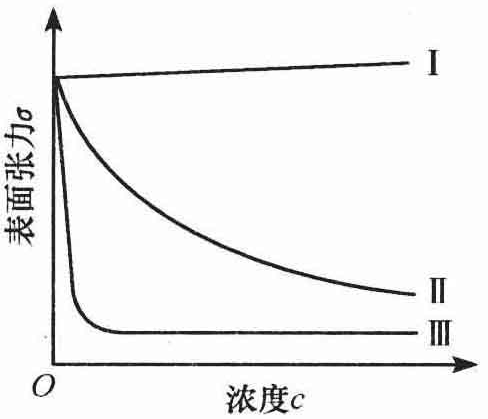
\includegraphics[width=\linewidth]{figures/fig8.6.png}
        \end{minipage}

\end{frame}


\begin{frame}
    \frametitle{吉布斯吸附定温式}

    溶液表面层与体相溶液组成不同的现象称为溶液表面吸附。
    \begin{itemize}
      \item 溶质在表面相浓度高于液相内部，使溶液的表面张力降低
      \item 溶质在表面相浓度低于其在液相内部的浓度，使溶液的表面张力升高
    \end{itemize}

    吉布斯用热力学方法导出了一定温度下，联系溶液的表面张力、溶液浓度和吸附量的微分方程，通常称为吉布斯吸附定温式。
    \[
        \varGamma =-\frac{c}{R T}\left(\frac{\partial \sigma}{\partial c}\right)_{T}
    \]
    $\varGamma$为单位面积表面相中吸附溶质的过剩量，又称表面过剩量。
    
    \begin{itemize}
        \item 若$\left(\frac{\partial \sigma}{\partial c}\right)_{T}<0$， 则$\varGamma > 0$。表面张力随着溶质的加入而降低者，是正吸附。
        \item 若$\left(\frac{\partial \sigma}{\partial c}\right)_{T}>0$， 则$\varGamma < 0$。表面张力随着溶质的加入而升高者，是负吸附。
    \end{itemize}
\end{frame}


\begin{frame}
    \frametitle{吸附量与浓度的关系}

    一定温度下实验测定不同浓度$c$对应的溶液表面张力值$\sigma$。以$\sigma$对$c$作图，在$\sigma - c$曲线上作切线，指定浓度下切线的斜率即为该浓度的$\left(\frac{\partial \sigma}{\partial c}\right)_{T}$值，再由吉布斯吸附定温式，即可得浓度时的表面吸附量$\varGamma$。作$\varGamma - c$曲线，称为吸附定温线。

        \begin{minipage}{0.61\linewidth}
            \begin{itemize}
                \item 溶质浓度很小时，$\varGamma$与$c$的关系近似直线，吸附量随溶质浓度的增加而增大；
                \item 当浓度足够大时，表面吸附量趋近一极限值$\varGamma_\mathrm{m}$，此时溶液表面的吸附已达饱和。
                \item 再增加浓度，表面吸附量不再改变，$\varGamma_\mathrm{m}$为一定值，与浓度无关。$\varGamma_\mathrm{m}$称为饱和吸附量。
            \end{itemize}
        \end{minipage}\hfill
        \begin{minipage}{0.37\linewidth}
            \begin{figure}[htpb]
                \centering                
                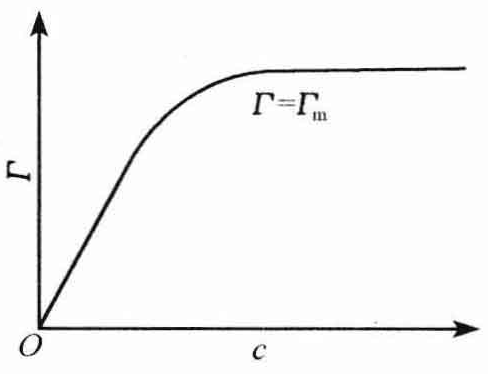
\includegraphics[width=.9\linewidth]{figures/fig8.7.png} 
                \caption{表面活性物质的吸附定温线}
            \end{figure}
        \end{minipage}

\end{frame}


\begin{frame}
    \frametitle{吸附层上分子的定向排列}

    表面活性物质分子具有两亲特性，分子的一端是亲油的非极性基团，另一端是极性基团，其亲水作用使分子的极性端进入水中。当浓度较高，溶质分子在表面层达饱和吸附时，分子在表面定向排列成单分子膜。
    \begin{figure}[htpb]
        \centering
        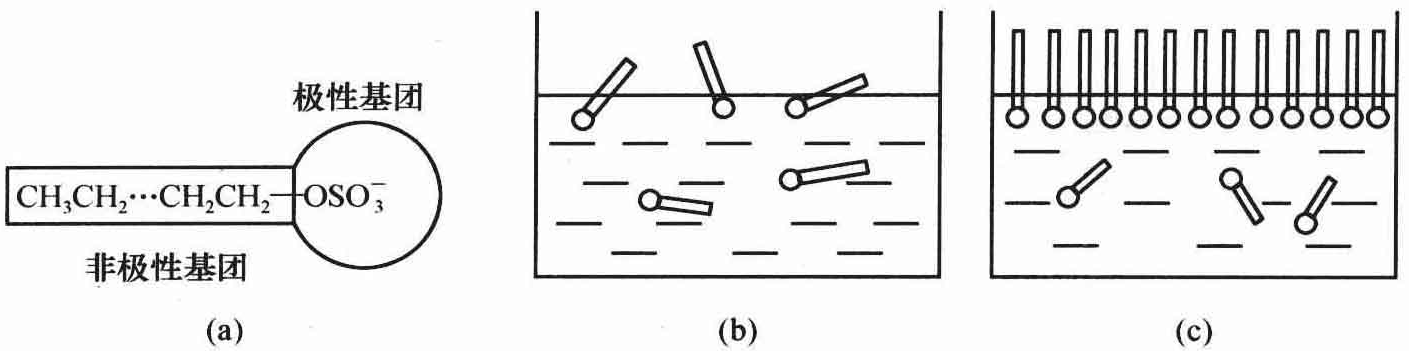
\includegraphics[width=\linewidth]{figures/fig8.8.png}
    \end{figure}
    \[
       \text{分子截面积} \quad A = \frac{1}{L \varGamma_\mathrm{m}}
    \]

\end{frame}